

\section{Opciones}
Una \textbf{Call} option es el derecho a comprar un \textbf{underlying asset} por un \textbf{exercise/strike price} hasta o el \textbf{expiry/expiration date}.\ Una \textbf{put option} es lo mismo, pero te da derecho a vender. Muchas veces las opciones se agrupan en \textbf{series}, i.e.\ diferentes combinaciones de strike y vencimiento disponibles para un mismo activo. Su \textbf{payoff function} es:
\begin{itemize}
    \item \textbf{Call option}: Apuestas a que el mercado sube
    \[\boxed{\max(S-K, 0)}\]
    \begin{figure}[H]
        \centering
        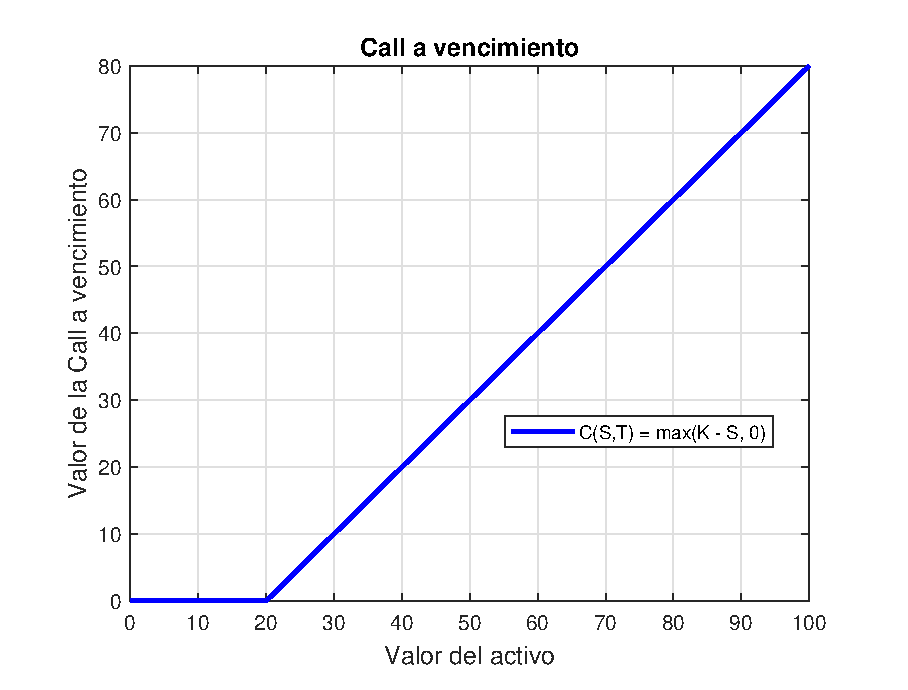
\includegraphics[width=0.5\linewidth]{Imagenes/2_Derivados/PayOffCall.eps}
        \caption{Payoff de opción Call a vencimiento}
    \end{figure}
    \item \textbf{Put option}: Apuestas a que el mercado baje
    \[\boxed{\max(K-S, 0)}\]
    \begin{figure}[H]
        \centering
        \includegraphics[width=0.5\linewidth]{Imagenes/2_Derivados/PayOffPut.eps}
        \caption{Payoff de opción Put a vencimiento}
    \end{figure}
\end{itemize}
A veces el strike $K$ se representa con una $E$. Las opciones \textbf{vainilla} son aquellas más simples; la función de pago solo depende del valor del subyacente en el momento del pago. Los \textbf{derivatives or contingent claims} son contratos que tienen dependencias más complejas.


\subsection{Terminología}
\begin{itemize}
    \item \textbf{Premium}: lo que se paga inicialmente por el contrato (prima).
    \item \textbf{Underlying (asset)}: subyacente sobre el que depende el contrato.
    \item \textbf{Strike (price)/exercise price}: precio al que se compra o vende el subyacente. Se define con $E$ o con $K$.
    \item \textbf{Expiration (date) o expiry (date)}: fecha en la que se puede ejercer o cuando se caduca la opción. Se denota por $T$.
    \item \textbf{Intrinsic value}: Valor del beneficio si la opción se ejerce en ese momento.
    \item \textbf{Time value}: Valor extra que tiene la opción por la incertidumbre futura.
    \item \textbf{In the money}: Opción con valor intrínseco positivo. Call: precio activo $>$ strike. Put: precio activo $<$ strike.
    \item \textbf{Out of the money}: Opción sin valor intrínseco. Call: precio activo $<$ strike. Put: precio activo $>$ strike.
    \item \textbf{At the money}: Precio del activo $\approx$ strike.
    \item \textbf{Long position}: Posición positiva en una cantidad o exposición.
    \item \textbf{Short position}: Posición negativa o venta en corto de un activo. ``Vender sin tener activo para adelantar dinero''.
    \item \textbf{Profit diagram}: Como el payoff, pero restandole la prima.
    \begin{figure}[H]
        \centering
        \begin{subfigure}[b]{0.45\linewidth}
            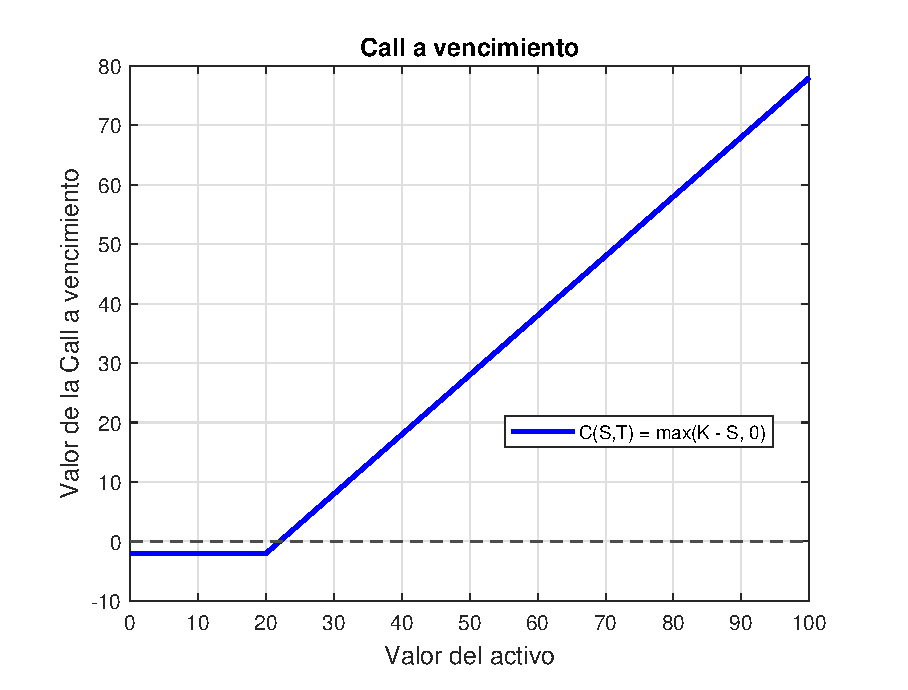
\includegraphics[width=\linewidth]{Imagenes/2_Derivados/ProfitDiagCall.eps}
            \caption{Call option}
        \end{subfigure}
            \begin{subfigure}[b]{0.45\linewidth}
            \includegraphics[width=\linewidth]{Imagenes/2_Derivados/ProfitDiagPut.eps}
            \caption{Put option}
        \end{subfigure}
        \caption{Profit diagram de opción a vencimiento}
    \end{figure}
    \item \textbf{Over the counter/OTC}: opciones que se realizan fuera de la bolsa y que no tienen que seguir las convenciones estándar. Los términos se especifican en una \textbf{term sheet}.
    \item \textbf{Gearing/leverage}: relación entre la posible ganancia y la inversión. Las opciones tienen una gran gearing, pero el punto negativo es que si no hay ganancias, la pérdida es del 100\% (se pierde la prima). Aquí el writer es el que tiene mucho riesgo.
    \item \textbf{Hedging}: tomar posiciones contrarias, por ejemplo ser el writer de una opción y comprar/vender acciones del subyacente para reducir riesgos. También se usa para describir la reducción de la aleatoriedad en general.
\end{itemize}



\subsection{Tipos de opciones}
\begin{itemize}
    \item \textbf{European options}: solo se puede ejercer en vencimiento.
    \item \textbf{American options}: se puede ejercer en cualquier momento hasta el vencimiento.
    \item \textbf{Bermudan options}: se puede ejercer en ciertas fechas específicas.
\end{itemize}


\subsection{Call-Put Parity}
La relación en cualquier tiempo $t$ entre una Call y una Put con los mismos parámetros es:
\[
    \boxed{C-P=S-Ke^{-r(T-t)}}
\]



\subsection{Opciones binarias/ digitales}
A fecha de ejercicio son discontinuas. Pagan una cierta cantidad fija (como un \$1) si el subyacente está por encima/debajo de cierto precio de ejercicio $E$ (o $K$). Las vainilla tienen un potencial de ganancia ilimitado, mientras que las binarias están acotadas, porque las compras cuando crees que el crecimiento/bajada es limitado.
\begin{figure}[H]
    \centering
    \begin{subfigure}[b]{0.45\linewidth}
        \includegraphics[width=\linewidth]{Imagenes/2_Derivados/BinaryCall.eps}
        \caption{Call option}
    \end{subfigure}
        \begin{subfigure}[b]{0.45\linewidth}
        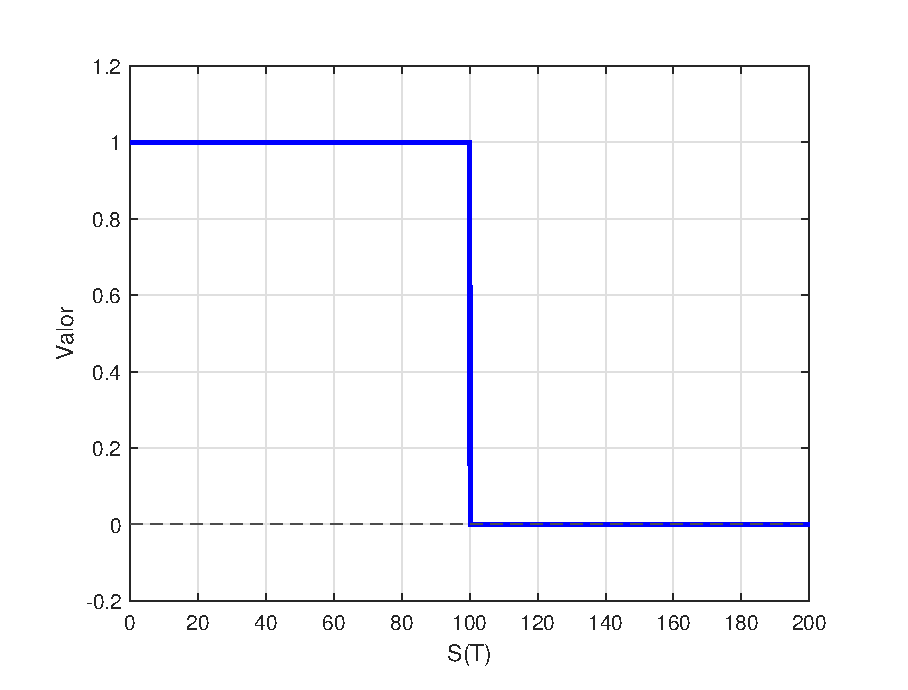
\includegraphics[width=\linewidth]{Imagenes/2_Derivados/BinaryPut.eps}
        \caption{Put option}
    \end{subfigure}
    \caption{Binary option payoff}
\end{figure}
Su relación de paridad se obtiene considerando que tienes una opción binary de cada tipo, porque a precio de ejercicio se obtiene el \$1 que se paga (o la cantidad que se haya firmado) actualizado:
\[\text{Binary call} + \text{Binary put} = e^{-r(T-t)}\]




\subsection{Portfolio of options/Option strategy}
Conjunto de opciones combinadas de manera estratégica para un objetivo concreto (maximizar ganancias, minimizar riesgos,\dots). Para saber su payoff se suman los payoff de las opciones que compras y se restan los payoff de las opciones que vendes. De forma genérica, las estrategias se pueden clasificar en \textbf{spread} que son estrategias que involucran opciones del mismo tipo (calls o puts), y \textbf{combinations} que combinan opciones de distinto tipo (calls o puts); también existen las \textbf{calendar spread}, que combinan opciones con distintas fechas de vencimiento. Algunos ejemplos son:
\begin{itemize}
    \item \textbf{Bull Spread (Spread Alcista)}: consiste en comprar una opción \textbf{call} con un strike más bajo $E_1$ y veneder otra opción call con strike más alto $E_2$  ($E_1<E_2$). Hay beneficio si subyacente \textbf{sube}, pero está limitado a diferencia $E_2-E_1$. Su payoff es:
    \[\boxed{\max(S-E_1, 0) - \max(S-E_2, 0)}\]
    \begin{figure}[H]
        \centering
        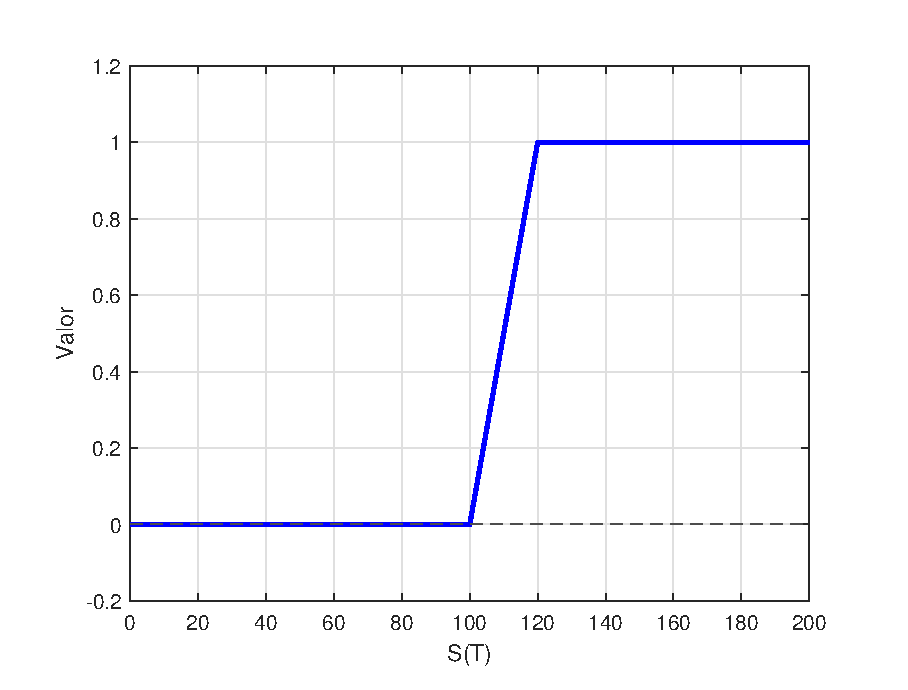
\includegraphics[width=0.5\linewidth]{Imagenes/2_Derivados/BullPayoff.eps}
        \caption{Payoff de Bull Spread a vencimiento (normalizado)}
    \end{figure}
    Para normalizarlo se divide por $E_2-E_1$
    \item \textbf{Bear Spread (Spread Bajista)}: consiste consiste en comprar opción \textbf{put} con strike más alto $E_2$ y vender otra con strike más bajo $E_1$ ($E_1<E_2$). Hay beneficio si el subyacente \textbf{baja}, pero está limitado a diferencia $E_2-E_1$. Su payoff es:
     \[\boxed{\max(E_2-S, 0) - \max(E_1-S, 0)}\]
    \begin{figure}[H]
        \centering
        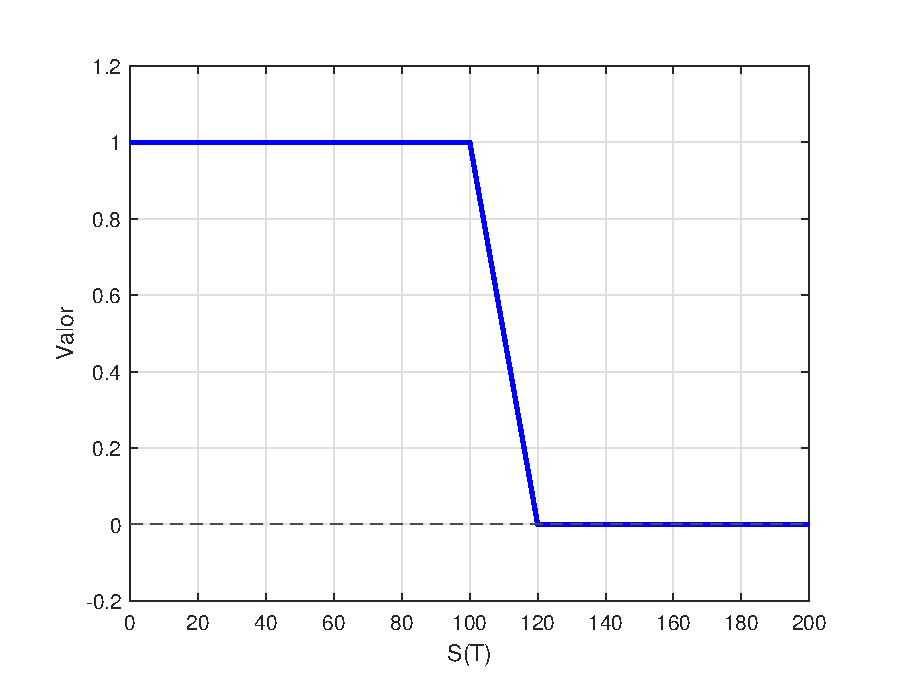
\includegraphics[width=0.5\linewidth]{Imagenes/2_Derivados/BearPayoff.eps}
        \caption{Payoff de Bear Spread a vencimiento (normalizado)}
    \end{figure}
    Para normalizarlo se divide por $E_2-E_1$
    \item \textbf{Straddles}: comprar una call y una put con mismo strike y mismo expirity. Beneficio depende de la magnitud del movimiento del subyacente, pero costo alto por primas de dos opciones. Se suele hacer cuando hay un anuncio importante. Su payoff es:
    \[\boxed{\max(S-E, 0) + \max(E-S, 0)}\]
    \begin{figure}[H]
        \centering
        \includegraphics[width=0.5\linewidth]{Imagenes/2_Derivados/StraddlePayoff.eps}
        \caption{Payoff de Straddle}
    \end{figure}
    \item \textbf{Strangle}: similar a straddles, pero con strikes distintos. Es más barato pero precisa de mayores cambios en el subyacente para que haya beneficios. Su payoff es:
    \[\boxed{\max(S-E_C, 0) + \max(E_P-S, 0)}\]
    Según los strikes pueden ser:
    \begin{itemize}
        \item \textbf{Out-of-the-Money Strangle (OTM)}: se compra call con strike por encima de precio actual y put con strike por debajo de actual. Es más barato (primas bajas) pero se necesita un movimiento grande del subyacente.
        \begin{figure}[H]
            \centering
            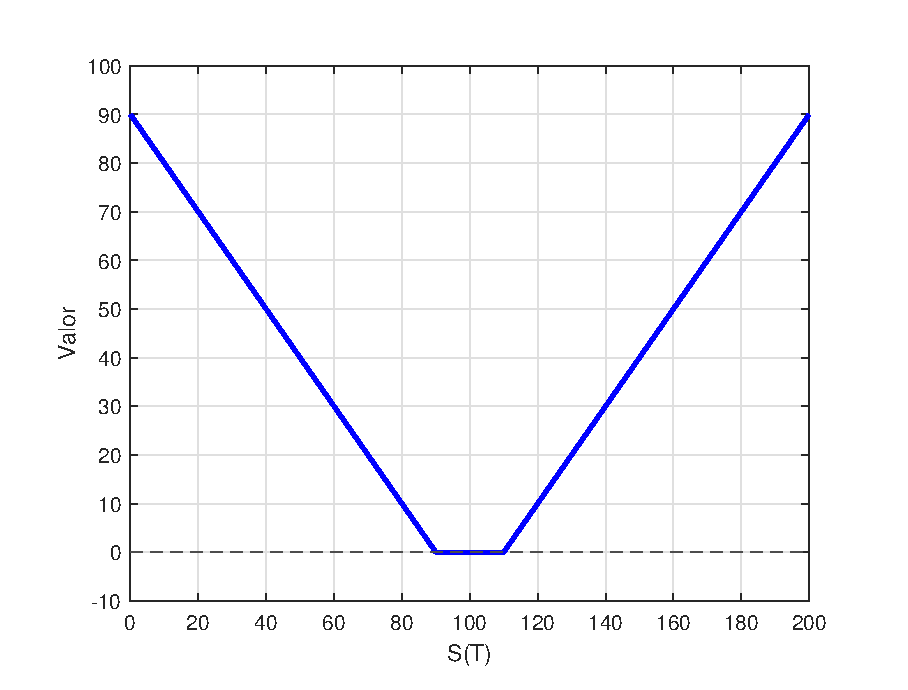
\includegraphics[width=0.5\linewidth]{Imagenes/2_Derivados/StrangleOTMPayoff.eps}
            \caption{Payoff de Strangle OTM}
        \end{figure}
        \item \textbf{In-the-Money Strangle (ITM)}: se compra call con strike por debajo de precio actual y put con strike por encima de actual. Algo más caro (por primas) que OTM, pero un poco más seguro.
        \begin{figure}[H]
            \centering
            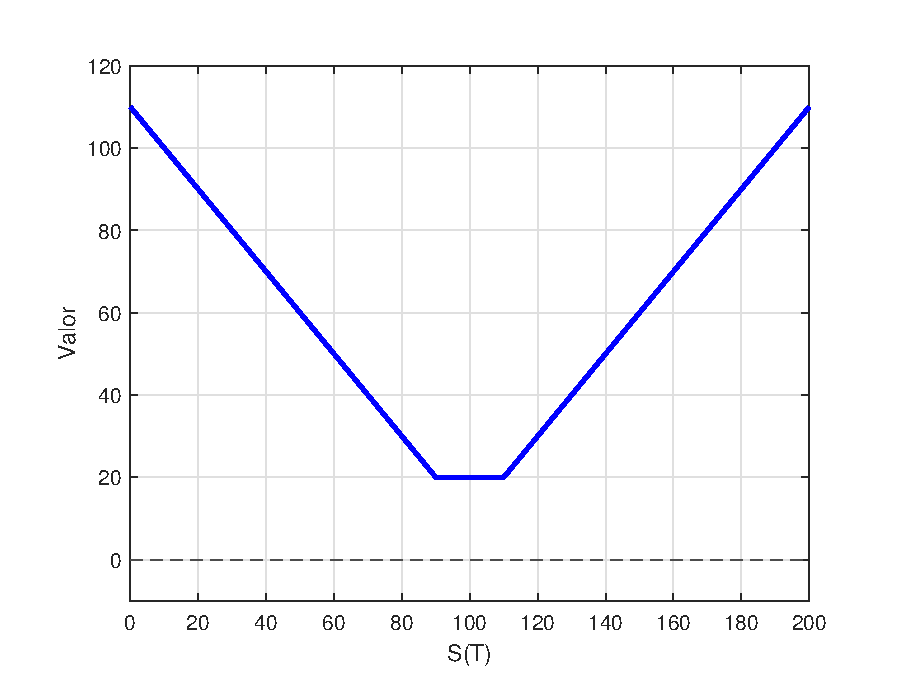
\includegraphics[width=0.5\linewidth]{Imagenes/2_Derivados/StrangleITMPayoff.eps}
            \caption{Payoff de Strangle ITM}
        \end{figure}
    \end{itemize}
    \item \textbf{Risk Reversal}: comprar una call con strike mayor que el precio actual y vender una put con un strike inferior al precio actual. Se apuesta a que el subyacente va a subir (y que como mucho no va a bajar demasiado). Si el activo baja se pierde dinero, pero las primas son más baratas. Su payoff sería:
    \[\boxed{\max(S-E_C, 0) - \max(E_P-S, 0)}\]
    \begin{figure}[H]
        \centering
        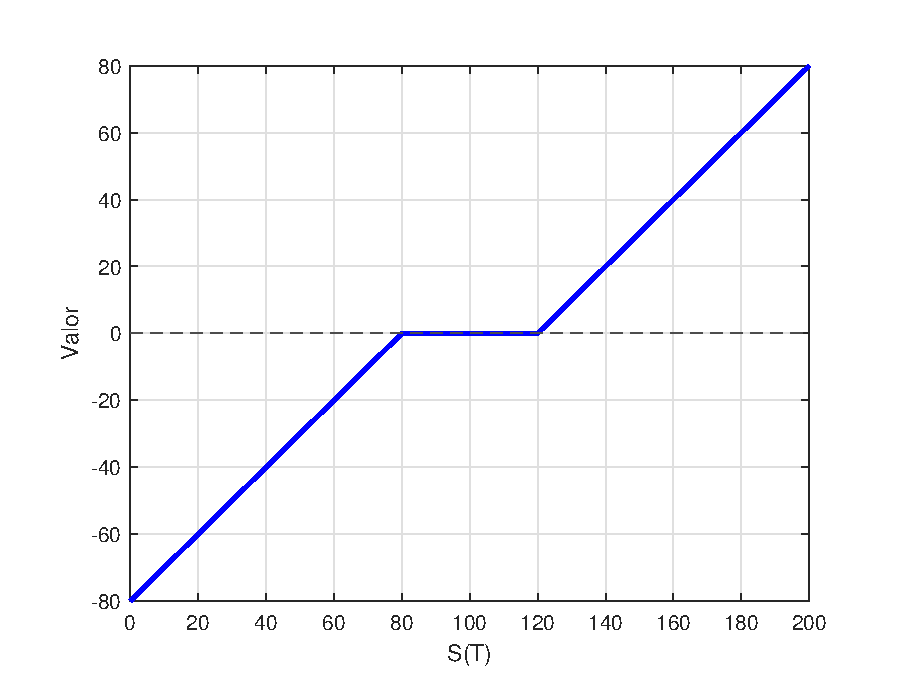
\includegraphics[width=0.5\linewidth]{Imagenes/2_Derivados/RiskReversalPayoff.eps}
        \caption{Payoff de Risk Reversal a vencimiento}
    \end{figure}
    \item \textbf{Butterflies}: se compra una call ITM ($E_{C_{ITM}}$), se venden dos calls ATM (at-the-money) ($E_{C_{ATM}}$) y se compra una call OTM ($E_{C_{OTM}}$). Es decir, $E_{C_{ITM}}<E_{C_{ATM}}<E_{C_{OTM}}$. Además, generalmente se cumple que $E_{C_{OTM}} - E_{C_{ATM}} = E_{C_{ATM}} - E_{C_{ITM}}$. Se usa cuando se espera que el subyacente esté cerca de cierto precio central y haya poca volatilidad. Su payoff es:
    \[\boxed{\max(S-E_{C_{ITM}}, 0) - 2\max(S-E_{C_{ATM}}, 0) + \max(S-E_{C_{OTM}}, 0)}\]
    \begin{figure}[H]
        \centering
        \includegraphics[width=0.5\linewidth]{Imagenes/2_Derivados/ButterflyPayoff.eps}
        \caption{Payoff de Butterfly a vencimiento}
    \end{figure}
    \item \textbf{Condors}: parecido a butterflies, se compra call con strike $E_1$, se vende call con strike $E_2$, se vende call con strike $E_3$, y se compra call con strike $E_4$ tal que $E_1<E_2<E_3<E_4$. Además, generalmente se cumple que $E_2-E_1=E_4-E_3$. Se obtienen ganancias máximas si el subyacente se mantiene entre $E_2$ y $E_3$. Su payoff es:
    \[\boxed{\max(S-E_1, 0) - \max(S-E_2, 0) - \max(S-E_3, 0) + \max(S-E_4, 0)}\]
    \begin{figure}[H]
        \centering
        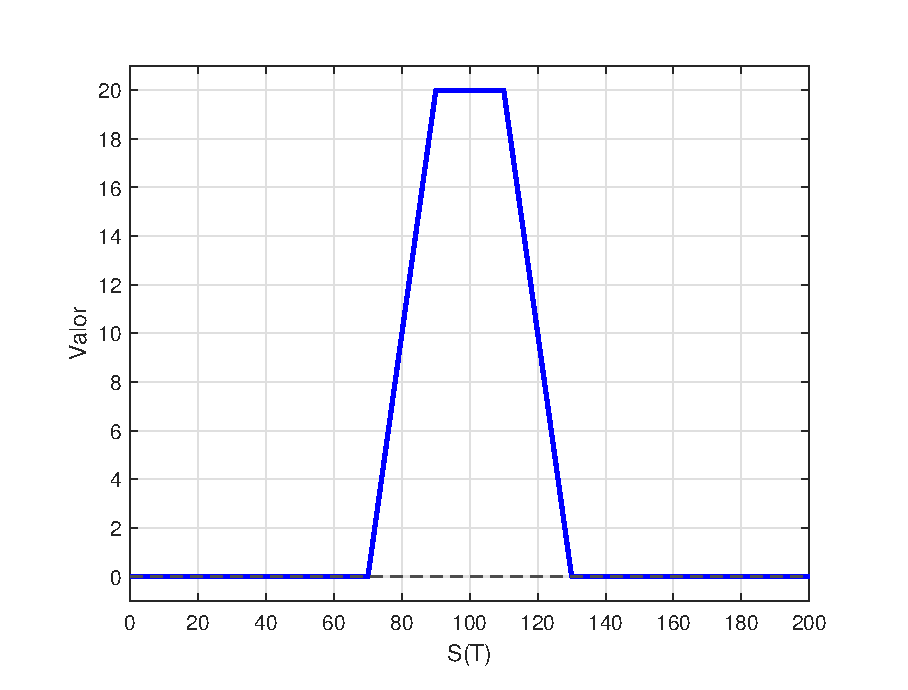
\includegraphics[width=0.5\linewidth]{Imagenes/2_Derivados/CondorsPayoff.eps}
        \caption{Payoff de Condors a vencimiento}
    \end{figure}
\end{itemize}



\subsection{Opciones a largo plazo}
\begin{itemize}
    \item \textbf{LEAPS/ long-term equity anticipation securities}: opciones con hasta 3 años de fecha de vencimiento. Usualmente vencen en enero. Se suelen emitir a 3 precios de ejercicio: ATM (precio actual), 20\% ITM (más favorable para el comprador) o 20\% OTM (más especulativo).
    \item \textbf{FLEX/ FLexible EXchange-traded options}: permiten más personalización de la opcion de la fecha de vencimiento (hasta 5 años), el strike o el tipo de ejercicio (europeo o americano).
\end{itemize}


\subsection{Otros derivados}
\begin{itemize}
    \item \textbf{Warrants}: parecido a opciones call, pero emitido por la propia empresa del subyacente que da derecho a comprar acciones \textit{nuevas} (frente a acciones ya existentes en las opciones) emitidas por la empresa. Tiene plazos largos, de hasta 5 años.
    \item \textbf{Convertible bonds/ CBs}: bono normal que paga cupones y un capital a vencimiento, pero que tiene la opción de convertirse en acciones antes de vencimiento (perderías los cupones siguientes). Se comporta como una opción americana.
\end{itemize}










